
\section{Experimental Setup}
The experiment was carried out at the Idaho Accelerator Center (IAC), using their fast-pulsed linear accelerator, which is an L--band frequency (1300 MHz) accelerator.
It is capable of pulse widths ranging from 50 ps to 2 $\mu$s with a maximum energy of 44 MeV.
See section~\ref{beam} for the accelerator parameters used during the experiment.
Figure~\ref{fig:Facility} shows a top down diagram of the experimental arrangement.

\begin{figure}[h]
\centering
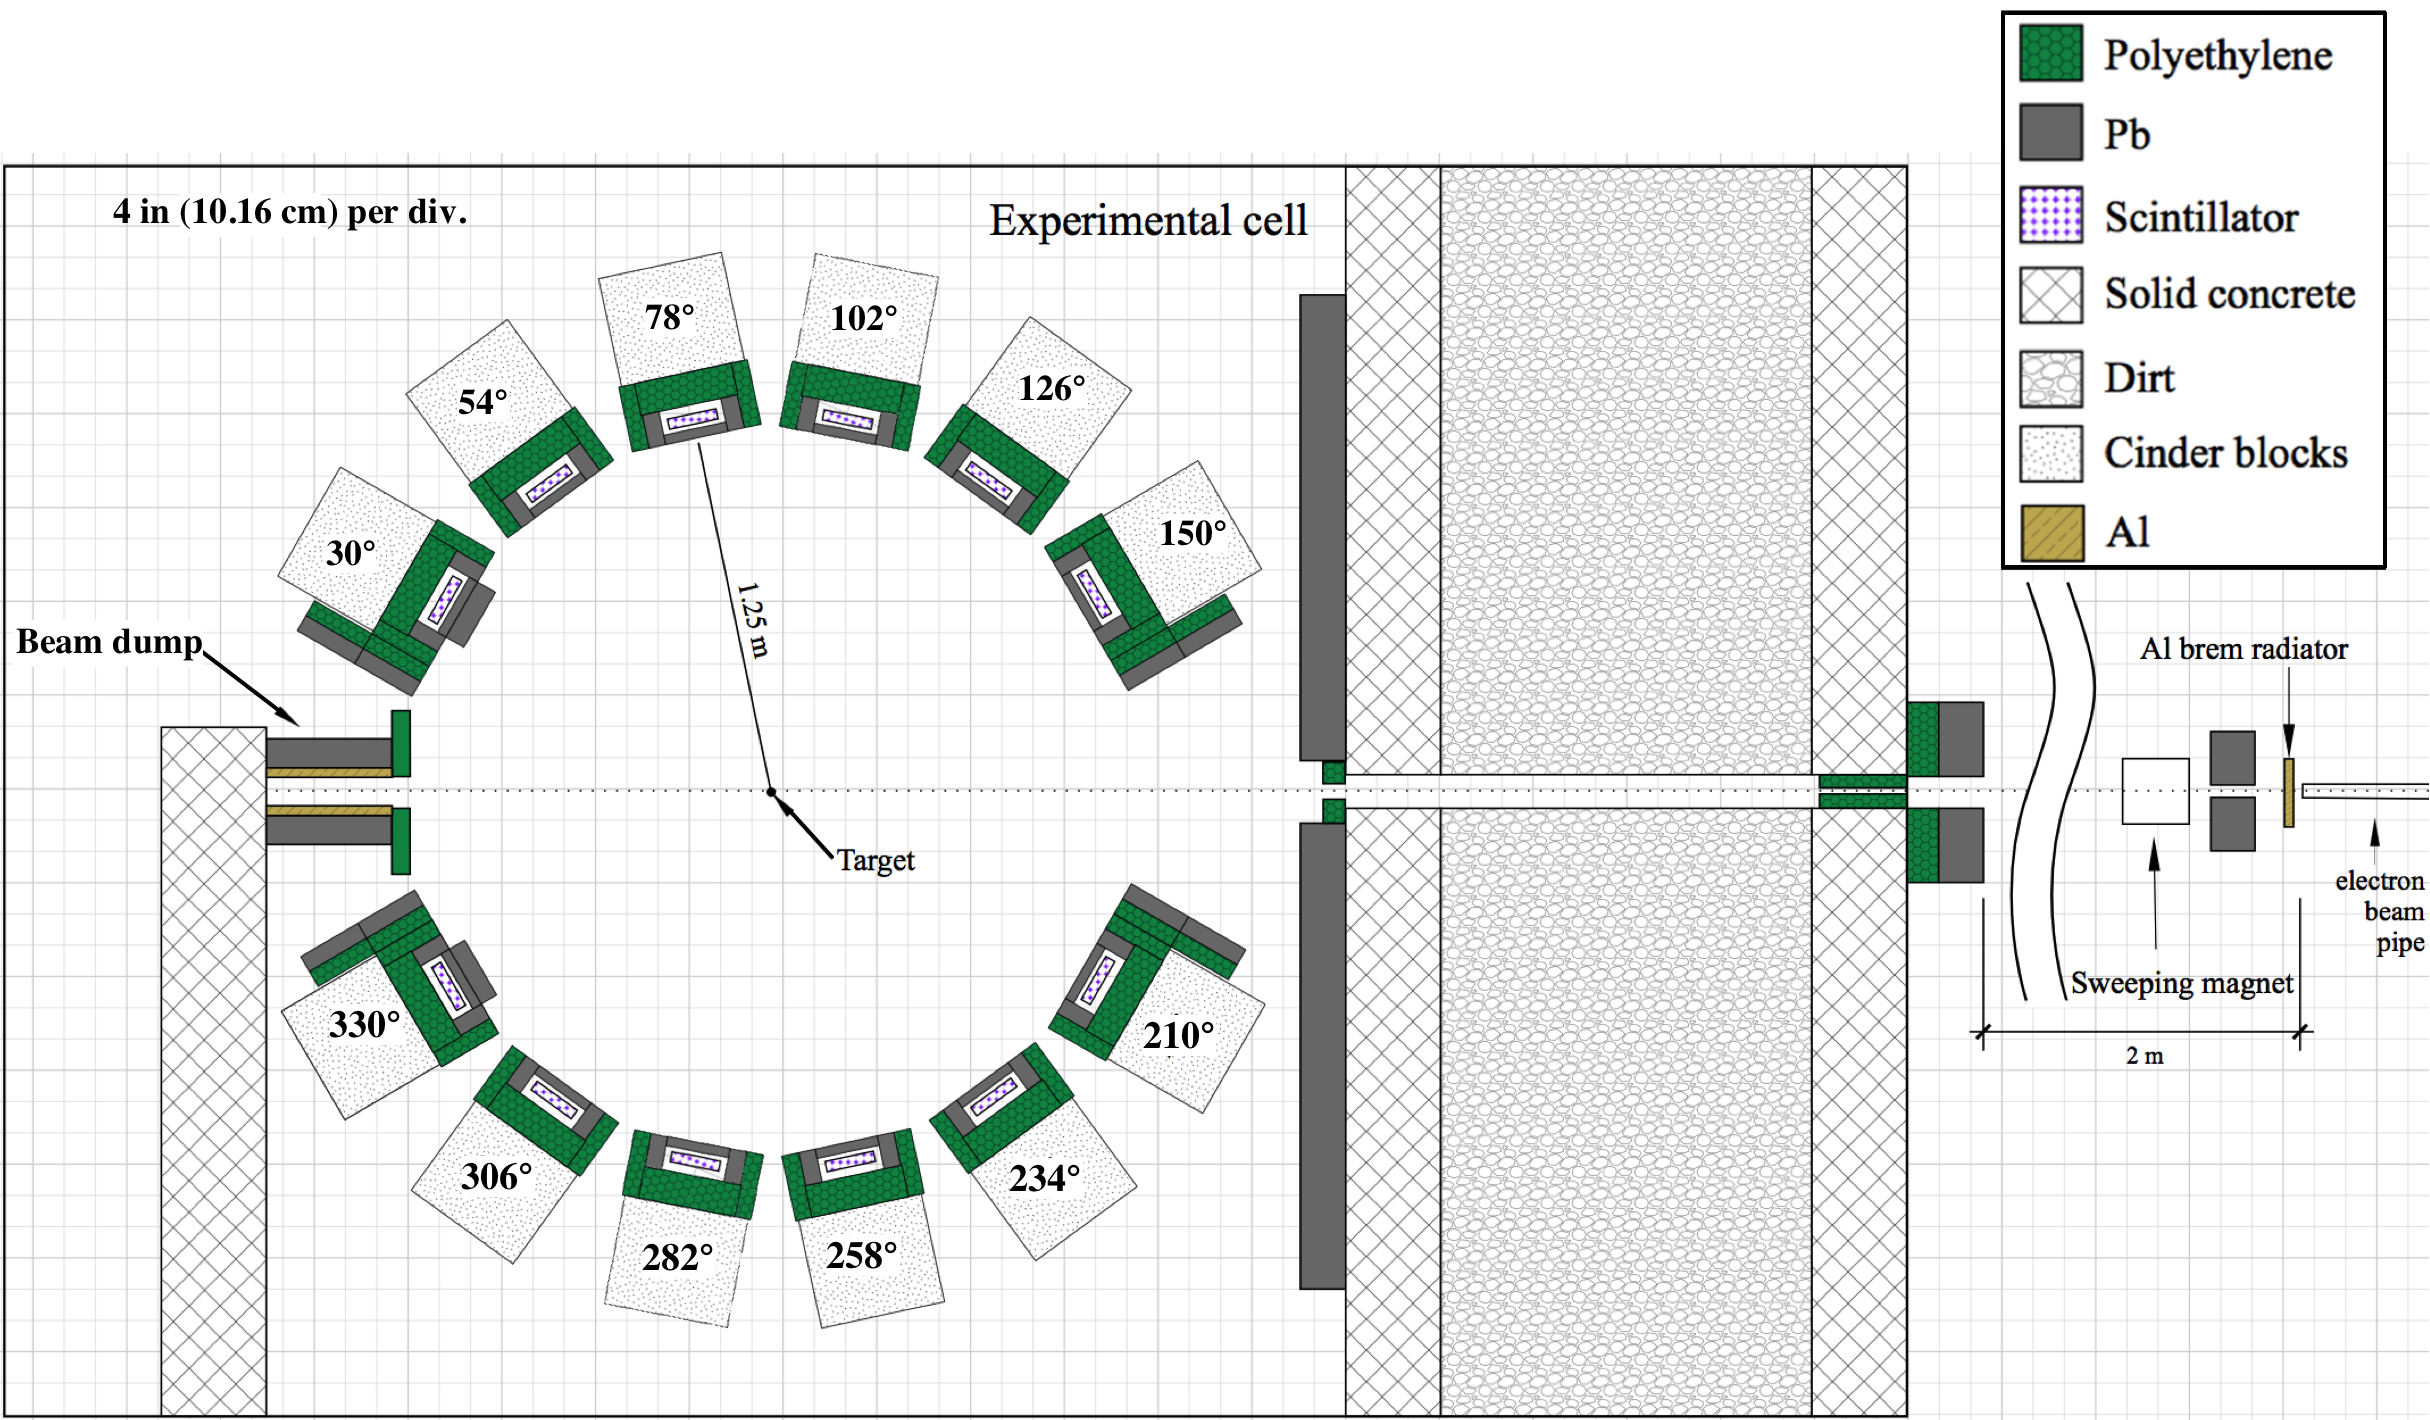
\includegraphics[width=0.95\textwidth]{Content/Methods/ExpArangment.jpg}
\caption{To-scale, top down diagram of the experimental setup.
An electron beam impinges upon a 3.8 cm thick Al radiator, and the resulting bremsstrahlung beam enters the experimental cell from the top.
The supporting structure for each detector has been labeled according to the angle, in degrees, between the center of each detector and direction of the incoming photon beam.
}
\label{fig:Facility}
\end{figure}
\subsection{Detectors}
\label{subsection:detectors}
The detection system measures neutron position and time of flight (ToF), which is defined as the time taken for a particle to travel from the target to any detector.
The purpose of ToF measurement is to calculate the kinetic energy of detected neutrons and to distinguish between photons and neutrons.
The neutron detection system consists of fourteen shielded scintillators arranged in a ring around the target (see Fig.~\ref{fig:DetGeom}).
The scintillators were made from Polyvinyl Toluene (PVT), an organic plastic scintillator.
Attached to both ends of each scintillator are 10-cm long, non-scintillating, ultra-violet transmitting light guides.
A Hamamatsu 580-17 photomultiplier (PMT) tube is fixed to each light guide using optical glue.
In order to increase the chance that scintillation light remains inside the scintillator, they were polished to remove micro-imperfections and were wrapped in reflective aluminized mylar.

\begin{figure}[]
    \centering
    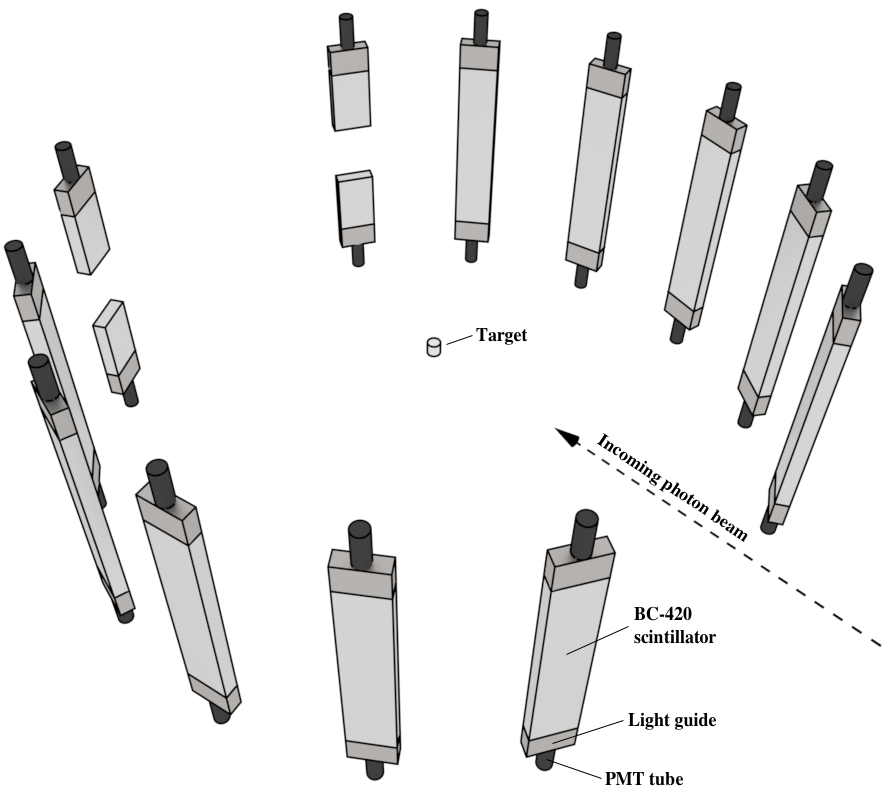
\includegraphics[width = 0.9\textwidth]{Content/Methods/Detectors.png}
    \caption{3-D render of the bare, unshielded scintillators, along with PMTs and light guides.}
    \label{fig:DetGeom}
\end{figure}

Ten out of the fourteen scintillators had dimensions of 76.2$\times$15.2$\times$3.8 cm$^3$.
The remaining four scintillators, with dimensions of 25.4$\times$15.2$\times$3.8 cm$^3$, were located at 30$^{\circ}$ and 330$^{\circ}$ with respect to the beam.
These scintillators were segmented in order to address very high photon detection rates resulting from the forward scattering of photons from the target.
Prior to segmentation, a photon was registered in these detectors nearly every pulse, and because the electronics were operated in single hit mode, the detection of a photon leaves the detector unable to detect subsequent neutrons, reducing the neutron detection efficiency to nearly 0\%.
After segmentation, the photon detection rate fell to 0.5 photons per pulse, greatly improving detector live-time.
The detectors at $\pm$30 degrees also differ from the rest in that they were instrumented with only a single PMT, and therefore have a lower position/energy resolution than the others.
In order to test for systematic errors that may have resulted from the use of the segmented detectors, opening angle measurements were compared with and without their use, and the differences were well within experimental errors.

The relative efficiencies of the neutron detectors as a function of neutron energy were calculated by diving measured and theoretical yields from the SF of $^{252}$Cf.
The results are shown in Fig.~\ref{fig:RelErgEfficiency}, which uses the aggregate of events from all detectors, and in Fig.~\ref{fig:RelErgEfficiencyVariation}, which shows it for each detector individually.
See section~\ref{Analysis} for a discussion on how the effects of detector efficiency are accounted for in this work.
\begin{figure}[]
    \centering
    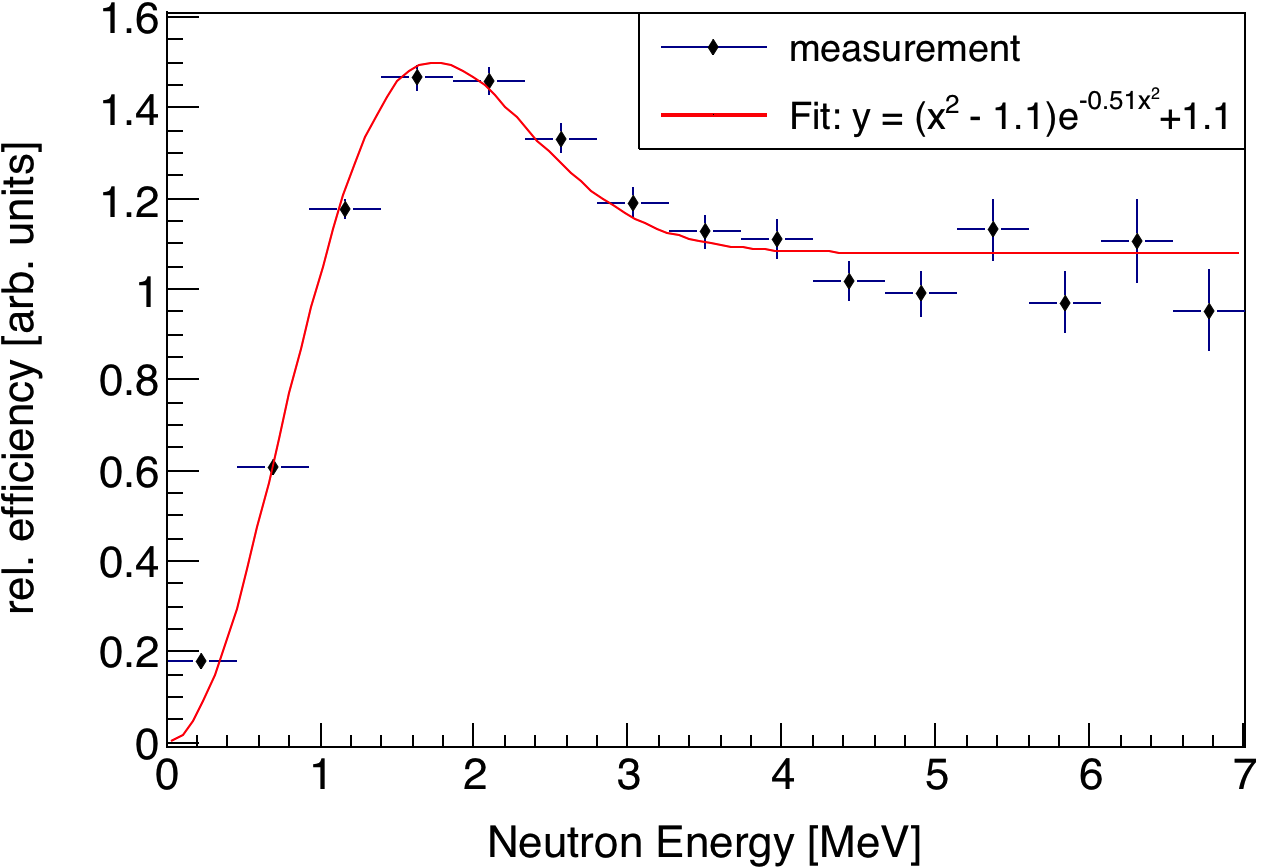
\includegraphics[width = 0.9\textwidth]{Content/Methods/RelErgEfficiency.png}
    \caption{The relative efficiency of the neutron detection system as a function of neutron energy is calculated by dividing the measured energy distribution by the theoretical energy distribution of neutrons from the SF of $^{252}$Cf.}
    \label{fig:RelErgEfficiency}
\end{figure}
\begin{figure}[]
    \centering
    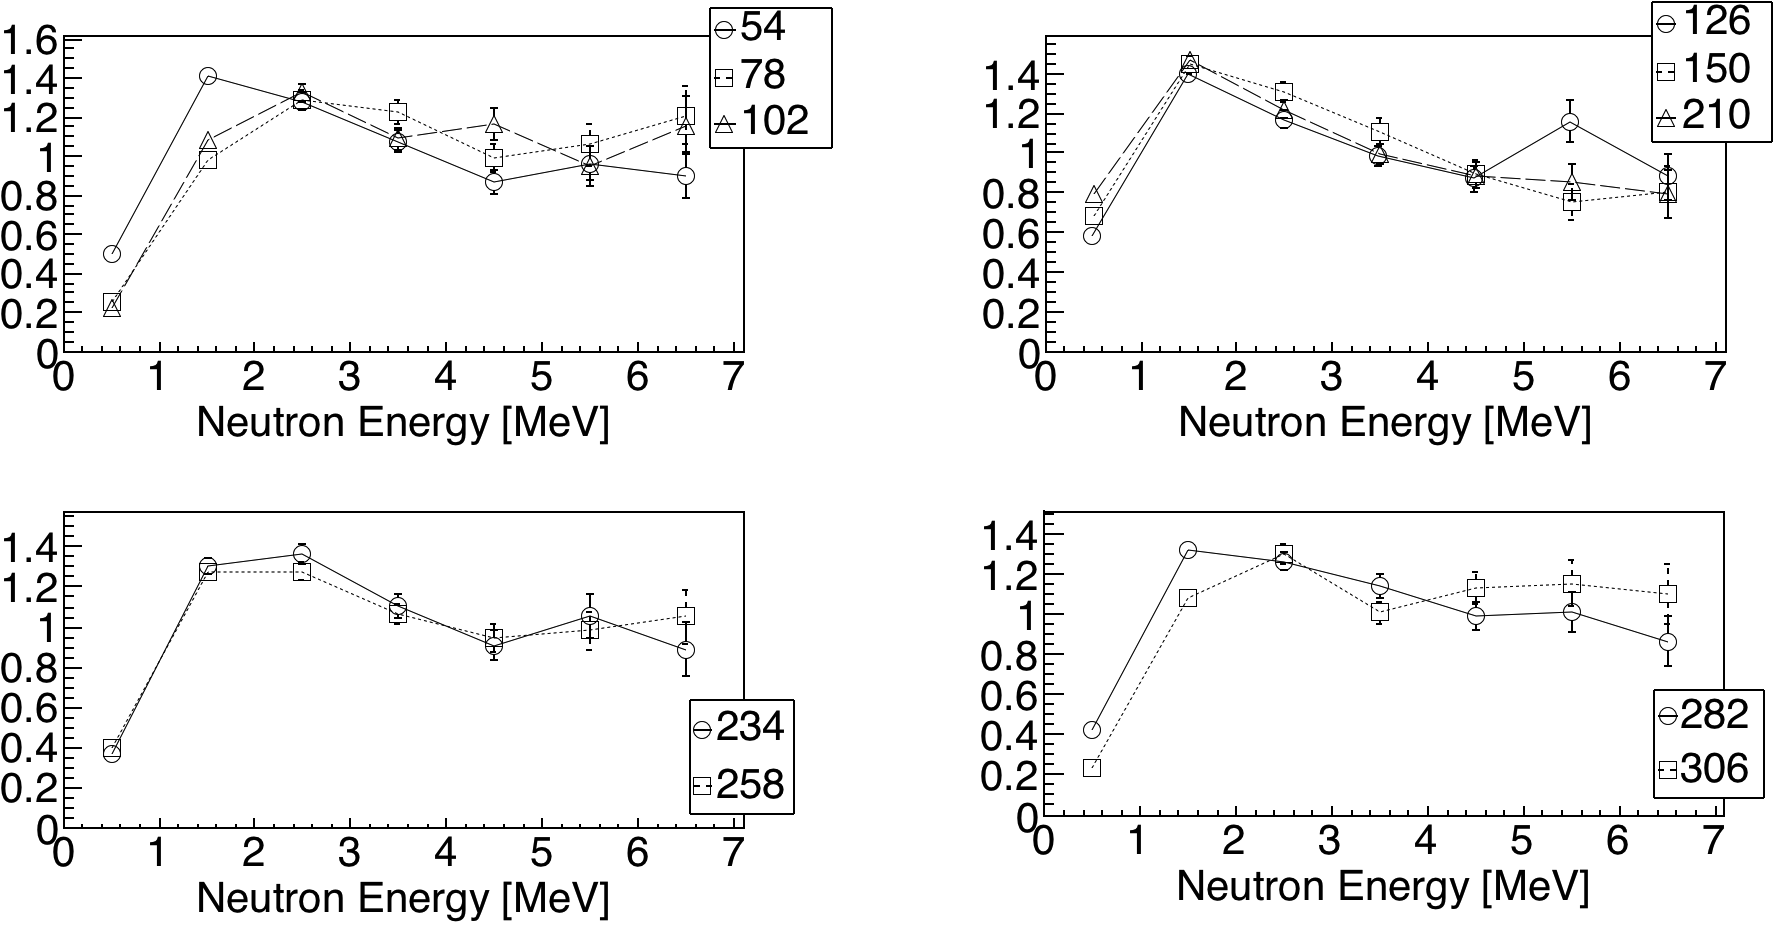
\includegraphics[width = 1\textwidth]{Content/Methods/RelErgEfficiencyVariation.png}
    \caption{
    The neutron detection efficiency as a function of neutron energy varies among the detectors, which are labeled in this figure according to the angle each detector from the direction of the Bremsstrahlung photon beam.}
    \label{fig:RelErgEfficiencyVariation}
\end{figure}

\subsection{Detector Shielding}
\label{shielding}
\begin{figure}
    \centering
    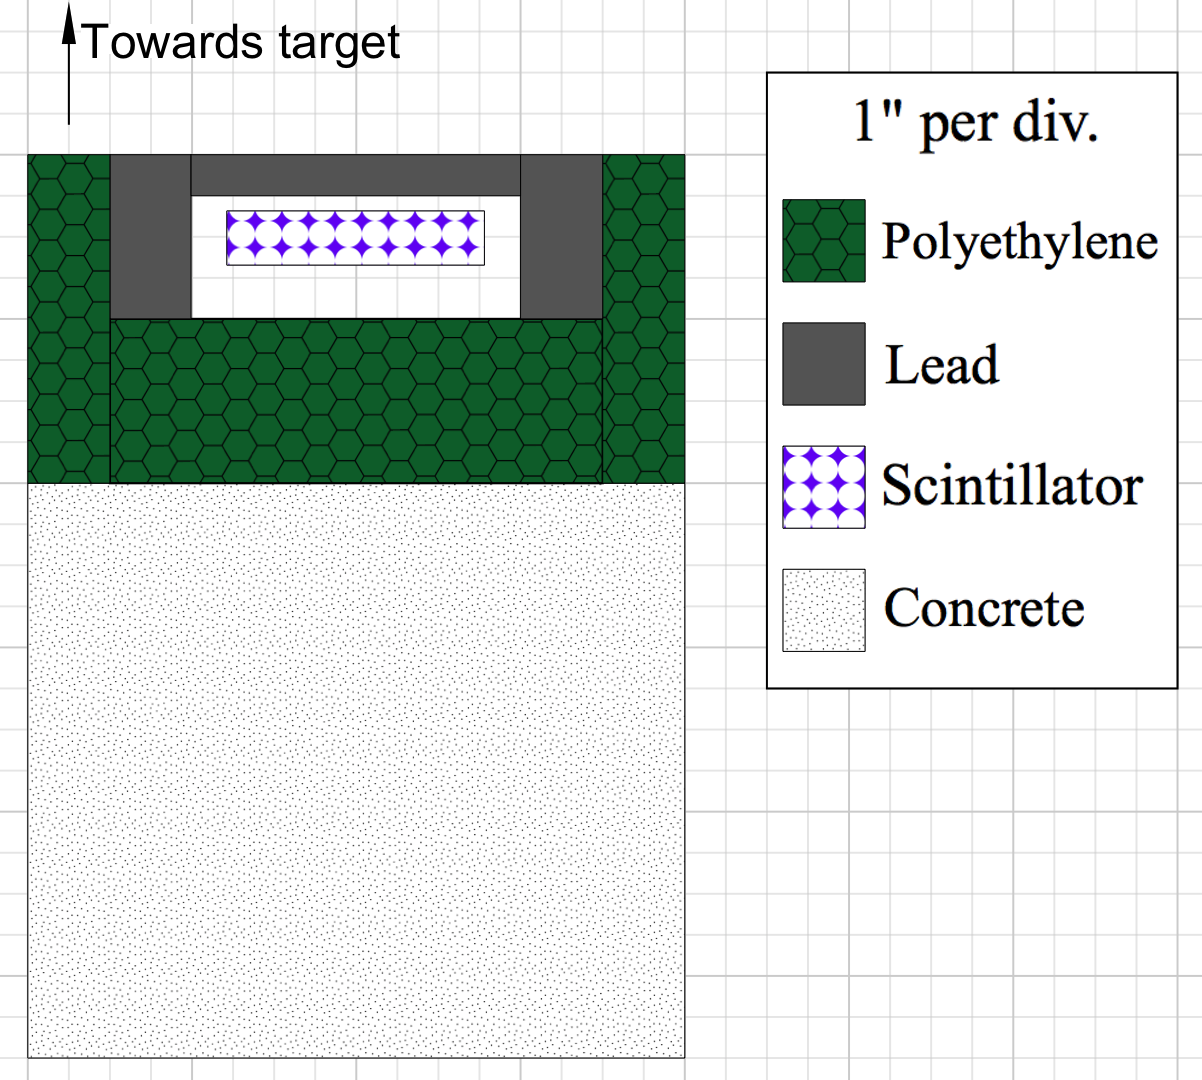
\includegraphics[width = 0.65\textwidth]{Content/Methods/DetShielding.png}
    \caption{Detector shielding was designed to reduce the detection of photons, room return, and detector cross-talk.}
    \label{fig:shielding}
\end{figure}
The detector shielding, depicted in Fig.~\ref{fig:shielding}, was constructed using lead and polyethylene with the aim of reducing cross-talk, the detection of photons, and noise.
Pb was used to attenuate photons, but has the side effects of neutron scattering and reduced neutron detection efficiency.
If a neutron scatters prior to being detected, the opening angle reconstruction and ToF calculation will be incorrect because both assume that detected neutrons travel a straight path from the target to the detector.
2.5~cm of Pb was placed along the front face of the scintillators, which is enough to largely reduce photon detection rates, and, according to an MCNP simulation, leads to a root-mean-square error in opening angle and ToF of 1$^{\circ}$ and 0.3~ns, respectively, due to neutron elastic scattering.
The sides of each scintillator were shielded with 5 cm of Pb to attenuate photons, followed by 5 cm of polyethylene to reduce the chance of neutron cross-talk.
Also in order to minimize cross-talk, Pb was not placed behind the scintillators after an MCNP-POLIMI simulation indicated it would occur at significant rates otherwise.
Instead, 10~cm of polyethylene was placed behind the scintillators.
For a more detailed discussion about the issue of cross-talk, see section~\ref{crosstalk}.

\subsection{Bremsstrahlung Photon Beam}
\label{beam}
In order to ensure that all correlated neutrons produced are due to fission, the bremsstrahlung end-point was set to 10.5~MeV, safely below the ($\gamma, 2n$) threshold of 11.28~MeV for $^{238}$U.
Al was chosen for a bremsstrahlung radiator, because Al has a neutron knockout threshold above the energy of the electron beam, which ensured that the radiator would not be a source of fast neutrons with the potential to interfere with the experiment.
Downstream from the bremsstrahlung radiator is a sweeping magnet to remove charged particles from the photon beam.
Next, the beam traveled through a series of polyethylene and lead collimators and into the experimental cell in which the target was located (see Fig.~\ref{fig:Facility}).
Figure~\ref{fig:BremDist} shows the energy distribution of photons that reach the target according to an MCNP simulation that included the production and collimation of the bremsstrahlung photon beam.

The electron beam pulse width was set to 3~ns with a repetition rate of 240~Hz and a 1.1~A peak current.
The 3~ns pulse width is not a large source of uncertainty in the measurement of neutron time of flight (ToF), because neutrons had a median ToF of $\approx$80~ns.

\begin{figure}[h]
\centering
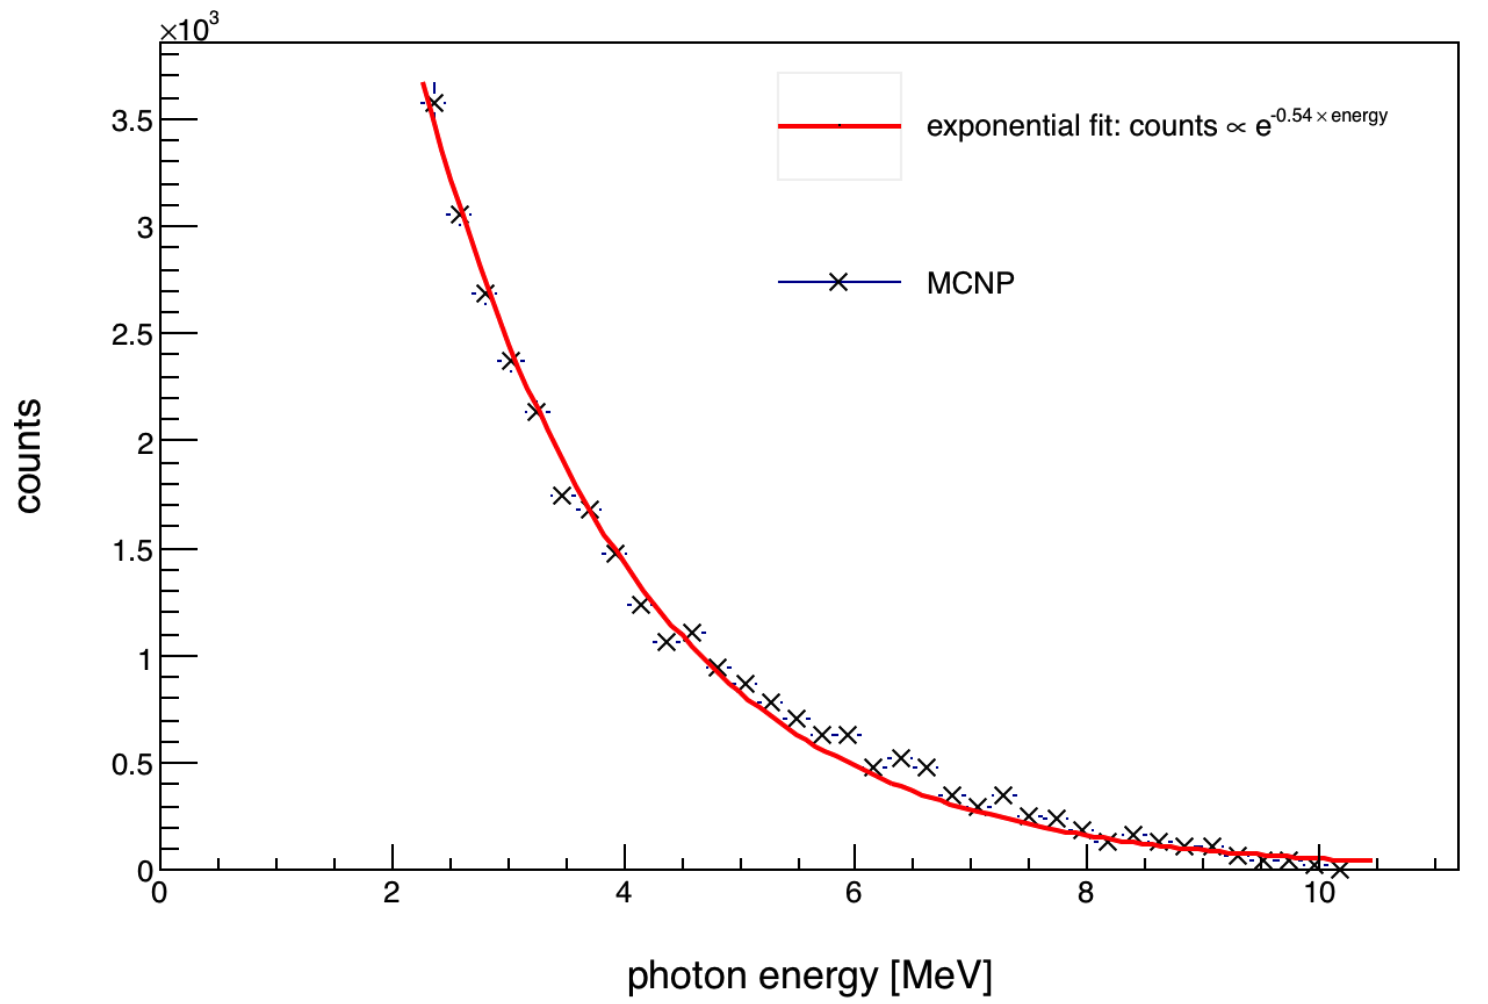
\includegraphics[width=0.7\textwidth]{Content/Methods/MCNPBremDistribution.png}
\caption{MCNP simulation of the energy distribution of photons that are incident on the fission target.}
\label{fig:BremDist}
\end{figure}
